%\VignetteIndexEntry{Ularcirc Vignette}
%\VignettePackage{Ularcirc}
%\VignetteEngine{knitr::knitr_notangle}


\documentclass[12pt]{article}\usepackage[]{graphicx}\usepackage[]{color}
%% maxwidth is the original width if it is less than linewidth
%% otherwise use linewidth (to make sure the graphics do not exceed the margin)
\makeatletter
\def\maxwidth{ %
  \ifdim\Gin@nat@width>\linewidth
    \linewidth
  \else
    \Gin@nat@width
  \fi
}
\makeatother

\definecolor{fgcolor}{rgb}{0.345, 0.345, 0.345}
\newcommand{\hlnum}[1]{\textcolor[rgb]{0.686,0.059,0.569}{#1}}%
\newcommand{\hlstr}[1]{\textcolor[rgb]{0.192,0.494,0.8}{#1}}%
\newcommand{\hlcom}[1]{\textcolor[rgb]{0.678,0.584,0.686}{\textit{#1}}}%
\newcommand{\hlopt}[1]{\textcolor[rgb]{0,0,0}{#1}}%
\newcommand{\hlstd}[1]{\textcolor[rgb]{0.345,0.345,0.345}{#1}}%
\newcommand{\hlkwa}[1]{\textcolor[rgb]{0.161,0.373,0.58}{\textbf{#1}}}%
\newcommand{\hlkwb}[1]{\textcolor[rgb]{0.69,0.353,0.396}{#1}}%
\newcommand{\hlkwc}[1]{\textcolor[rgb]{0.333,0.667,0.333}{#1}}%
\newcommand{\hlkwd}[1]{\textcolor[rgb]{0.737,0.353,0.396}{\textbf{#1}}}%
\let\hlipl\hlkwb

\usepackage{framed}
\makeatletter
\newenvironment{kframe}{%
 \def\at@end@of@kframe{}%
 \ifinner\ifhmode%
  \def\at@end@of@kframe{\end{minipage}}%
  \begin{minipage}{\columnwidth}%
 \fi\fi%
 \def\FrameCommand##1{\hskip\@totalleftmargin \hskip-\fboxsep
 \colorbox{shadecolor}{##1}\hskip-\fboxsep
     % There is no \\@totalrightmargin, so:
     \hskip-\linewidth \hskip-\@totalleftmargin \hskip\columnwidth}%
 \MakeFramed {\advance\hsize-\width
   \@totalleftmargin\z@ \linewidth\hsize
   \@setminipage}}%
 {\par\unskip\endMakeFramed%
 \at@end@of@kframe}
\makeatother

\definecolor{shadecolor}{rgb}{.97, .97, .97}
\definecolor{messagecolor}{rgb}{0, 0, 0}
\definecolor{warningcolor}{rgb}{1, 0, 1}
\definecolor{errorcolor}{rgb}{1, 0, 0}
\newenvironment{knitrout}{}{} % an empty environment to be redefined in TeX

\usepackage{alltt}

\usepackage{multirow}
\usepackage{mdframed}
\usepackage{hyperref}
\usepackage{graphicx}
\graphicspath{ {figures/} }
\usepackage[export]{adjustbox}


\title{Ularcirc Package User Manual}
\author{David Humphreys\\
Victor Chang Cardiac Research Institute\\
University of New South Wales
}
\IfFileExists{upquote.sty}{\usepackage{upquote}}{}
\begin{document}

\maketitle

%VERSIONS:
\begin{center}
\textbf{Ularcirc v}0.1.0
\end{center}
@

\tableofcontents



%--------------------------------------------------------------------------------
%--------------------------------------------------------------------------------
\section{Overview} \label{sec:praeludium}
%--------------------------------------------------------------------------------
%--------------------------------------------------------------------------------

\indent Splicing is the removal of intronic sequences from a nascent pre-mRNA transcript resulting in the formation of mature mRNA. There are numerous mechanisms of splicing and is a regulated process that typically involves multiple RNA-binding proteins. In Eukaryotes splicing can result in gene isoforms, poly-cistronic transcripts, gene fusions and circular RNA (circRNA). \par
 The complexities of splicing  can be captured by RNA-Sequencing. Ularcirc is designed to work with the output generated from the STAR aligner which produces output files of detected splice junctions. Ularcirc provides visualisation and analysis tools for both forward canonical splice junctions (generated from mature mRNAs) and backsplice junctions (generated from circRNAs). Ularcirc dynamically generates visualisations, including the ability to a zoom to defined regions within a gene locus, and furthermore can extract the transcript sequence that spans specific exon junctions. \par
 Ularcirc can be operated on any computer setup that can run the R-programing languange. All operations proceed in real time via a menu driven interactive analysis where data tables and visualization are generated dynamically. Ularcirc does not require significant computational resources and is currently implemented to operate on one CPU thread. The saved project data sets are small (typically in the low MB range) which enables easy sharing of data files. Introductory tutorials on how to use Ularcirc can be found on youtube. \par
Ularcirc is comprised of numerous interactive screens that comprise of a main and side panel. The main panel allows the selection of one of four tabs which are titled ``Setup'', ``Project'', ``Gene\_View'', ``Genome\_View'', ``Junction\_View''. A different side panel exists for each main panel and display  specific options that help direct and assemble analysis. The main panel will display output relevant for each stage of circRNA analysis which this vignette describes in detail. Users should be aware that some analysis may take time to complete and floating status bars will notify of the progress.

%--------------------------------------------------------------------------------
%--------------------------------------------------------------------------------
\section{Preparing input data sets} \label{sec:prepare}
%--------------------------------------------------------------------------------
%--------------------------------------------------------------------------------

%----------
\subsection{Splice junction files} \label{sec:FSJfiles}
%----------
\indent Ularcirc requires canonical and chimeric splice junction output files generated from the STAR aligner which  MUST contain the default file extensions of SJ.out.tab and Chimeric.out.junction respectively. For detailed instructions on how to use the STAR aligner please visit url https: github alexdobin STAR . Note that the STAR aligner requires significant computational resources. There are publically available GALAXY resources to run STAR if you do not have access to other high performance computational resources (\url {https://usegalaxy.org}). \par
To generate the required chimeric junction files the following two parameters must be supplied to the STAR aligner. The numeric value provided to each parameter describes features used to detect chimeric reads and therefore may need to be altered to improve sensitivity and accuracy.

\begin{mdframed}--chimSegmentMin 15  --chimJunctionOverhangMin 15 \end{mdframed}

Ularcirc can only add files to individual projects via one upload. Attempting to upload multiple times will only result in previous upload being overwritten by the current upload. Individual or multiple samples are identified by a common file prefix. Therefore for a given project all splice junction files must be located in a common directory and have the appropriate file prefix. For example if the following files were uploaded into Ularcirc:

\begin{mdframed}
SRR12345678\_e17.5\_heart.Chimeric.out.junction \\
SRR12345678\_e17.5\_heart.SJ.out.tab \\
SRR87654321\_P10\_heart.Chimeric.out.junction \\
SRR87654321\_P10\_heart.SJ.out.tab
\end{mdframed}

The above example would result in two samples IDs being imported into Ularcirc, SRR123456768\_e17.5\_heart and SRR87654321\_P10\_heart. It is highly recommended to provide a descriptive name as Ularcirc provides no functionality at this time to rename samples. After files are uploaded the Project filename can be entered and saved. The STAR aligner can be instructed to assign a common prefix to output files. This can be specified with the following option:

\begin{mdframed} --outFileNamePrefix Type\_your\_prefix\_here \end{mdframed}


%----------
\subsection{Annotation databases} \label{sec:AnnotDB}
%----------

\indent Ularcirc can annotate backsplice and canonical splice junctions via integrating bioconductor databases. Three installations are required per organism, examples of the required datasets for mouse and human is shown below in table 1.

\noindent
\begin{tabular}{ |l|l|l| }
\hline
\multicolumn{3}{ |c| }{ Example Bioconductor datasets} \\
\hline Genome & Database type & Database name \\ \hline
\multirow{3}{*}{hg19} &
BSGenome & BSgenome.Hsapiens.UCSC.hg19 \\
& TxDb & TxDb.Hsapiens.UCSC.hg19.knownGene \\
& OrgDatabase & org.Hs.eg.db \\ \hline
\multirow{3}{*}{hg38} &
BSGenome & BSgenome.Hsapiens.UCSC.hg38  \\
& TxDb & TxDb.Hsapiens.UCSC.hg38.knownGene \\
& OrgDatabase & org.Hs.eg.db \\ \hline
\multirow{3}{*}{mm9} &
BSGenome & BSgenome.Mmusculus.UCSC.mm9  \\
& TxDb & TxDb.Mmusculus.UCSC.mm9.knownGene \\
& OrgDatabase & org.Mm.eg.db \\ \hline
\multirow{3}{*}{mm10} &
BSGenome & BSgenome.Mmusculus.UCSC.mm10  \\
& TxDb & TxDb.Mmusculus.UCSC.mm10.knownGene \\
& OrgDatabase & org.Mm.eg.db \\ \hline
\end{tabular}

%--------------------------------------------------------------------------------
%--------------------------------------------------------------------------------
\section{Workflow} \label{sec:workflow}
%--------------------------------------------------------------------------------
%--------------------------------------------------------------------------------
Ularcirc is designed to follow a logical systematic workflow which is broken down into five key steps. Each step is can be performed  via a tabs that can be selected via the main panel as shown in figure \ref{fig:UlarcircTabs}. The workflow commences on the left most tab (``setup'') which is  the initial screen displayed. The setup tab also  provides a quickstart guide that briely describes the workflow. This chapter provides a more in depth overview of each of these steps and users are encouraged to familiarise themselves with the contents of this chapter to make the most out of Ularcirc.

\begin{figure}[h]
  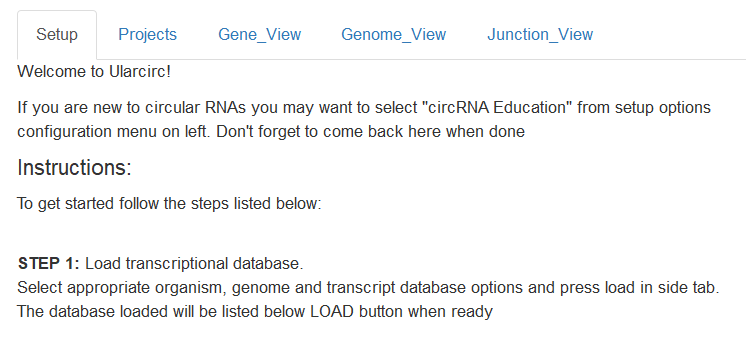
\includegraphics[width=\linewidth,frame]{MainPanelTabs}
  \caption { Screen shot of the five tabs that can be selected within Ularcirc }
  \label{fig:UlarcircTabs}
\end{figure}
%----------
\subsection{Step 1a: Loading annotation data} \label{sec:Step1a}
%----------
Upon startup Ularcirc loads and displays contents on the ``setup'' tab within the main panel. The side panel can be configured to one of three options which is selected via the pulldown menu under ``Step configuration''. The default configuration  is Load transcript database which enables the selection of organism, genome and transcriptome databases via separate pulldown menus under the heading ``ORGANISM''. If three pulldown menus are not populated this indicates that databases have not been installed from bioconductor.

%----------
\subsection{Step 1b: Setting filters} \label{sec:Step1b}
%----------
Ularcirc provides a number of filtering option that can be applied to datasets. Filter options can be found via the Setup tab on the main panel and selecting Load new data on the side bar panel. There are five filter options that all have default settings but can be adjusted by the user. Below is a descrition of each filter
 Same chromosomes  Selecting this checkbox will only select chimeric reads that span a common chromosome. At this point in time fusion circRNAs that span across multiple chromosomes are not supported. \par
Chimeric genomic distance   This is the maximum and minimum chimeric distance considered for chimeric junctions that are identified on the same chromosome. The default settings will not detect and chimeric junction that spans less than 200nt or longer than 100000nt. \par
 Same strand Will only select chimeric junctions that are from the same strand.
 DON'T remove any canonical junctions: The STAR aligner does occasionally report what appears to be a likely canonical junction within the chimeric junction output. This setting saves all candidates. \par
 Junction threshold Users can select backsplice junctions that have a minimum coverage. Te default setting is 1.
 RAD score The read alignment distribution (RAD) score is a metric that identified false positive chimeric reads. It is only applicable for paired end sequencing data. \par

It is important to note that the setting of these filters prior to uploading a new data set will not save  any chimeric junctions that do not pass filter settings. For exploratory analysis users may wish to relax some filter settings prior to saving and then explore more stringent filter settings thereafter. Finally the filters provided in Ularcirc only apply to chimeric junctions. At this point in time no filter applies to canonical forward junctions. \par

SINGLE END DATA SETS : The RAD filter should be set to 0 and 1 as this score cannot be applied. Failing to do this will results in no back splice junction detection.


%----------
\subsection{Step 1c: Loading new data sets} \label{sec:Step1c}
%----------
Ularcirc takes chimeric and canonical splice junction files as provided by the STAR aligner. Chimeric junction files must have the extension Chimeric out junction while canonical junctions must have the extension SJ out tab. The prefix of these files must be identical (explained in more detail below). To upload files users must navigate to the Setup tab and then select Load new data under the pull down menu Setup option configuration. Prior to file upload a number of genomic filtering configuration options are available. The default filters require that chimeric alignments exist on the same strand of the same chromosome and that the chimera junction occurs over a distance less than 100,000 nucleotides.  There are currently no filters for canonical splice junctions and Ularcirc will display information on unique splice junction alignments as provided by the STAR aligner. Once filters are defined the user then selects the upload button and files are uploaded and alignments that don’t match filter settings are removed.
\indent Multiple samples can be uploaded into Ularcirc but this can only be done in one upload event. Attempting to upload files separately will only result in previous upload being overwritten by the current upload. During a multi-file upload samples are identified by a common file prefix.  For example if the following files were uploaded into Ularcirc

\noindent
\begin{mdframed}
SRR12345678\_e17.5\_heart.Chimeric.out.junction \\
SRR12345678\_e17.5\_heart.SJ.out.tab            \\
SRR87654321\_P10\_heart.Chimeric.out.junction   \\
SRR87654321\_P10\_heart.SJ.out.tab
\end{mdframed}


The above example would result in two samples IDs being imported into Ularcirc, SRR123456768\_e17.5\_heart and SRR87654321\_P10\_heart. It is highly recommended to provide a descriptive name as Ularcirc provides no functionality at this time to rename samples.

After files are uploaded the Project filename can be entered and saved (refer Step2 Savind/loading a project).


%----------
\subsection{Step 2a: Saving/loading a project and grouping samples} \label{sec:Step2}
%----------
\indent New data sets or existing project data sets can be saved or loaded through the Projects tab. Data sets that are loaded through Ularcirc can be saved as a project file which can then be reloaded at a later date. Projects should be saved in a common folder/directory that exists on the local file system. This folder/directory is defined at the top of the  main page of the projects tab. This directory should NOT be set to the R Ularcirc library  directory as any future upgrades will overwrite pre-existing files. \par

Different RNA-Seq library prep kits are capable of capturing the same or opposing strand of RNA. Some kits are do not capture the strand of a RNA transcript. The top most panel on the side bar provides the opportunity to record this information. \par

All saved projects that are present in the working directory will be listed in the pulldown menu located under the blue "Load" title on sidebar. Note that any new data sets that may have been loaded in the current Ularcirc session will not be visable until Ularcirc is restarted. To load selecting the project name and press load. Data is loaded when sample names are listed on the main tab. \par

To save a project a unique project name must be entered into the sidebar under entry "Name of project" and then pressing the save button. Ularcirc will not overwrite an existing project file and will warn users if the entered name is not unique.
%----------
\subsection{Step 2b: Grouping samples} \label{sec:Step2}
%----------

\indent After loading a project file or uploading new junction data the associated sample IDs will be listed with checkboxes in two locations on the main tab. These two listings are referred to as "Selected samples" and "Data groupings" and provide provide flexibility in the way downstream analysis can be performed. \par

The first listing which is under ``Selected Samples'' provides users the option to analyse a subset of specific data sets to analyse. This option is useful to explore circRNA expression patterns in individual data sets that are available within a project. Data sets that are selected in this list are the only samples that contribute to the integrated genomic visualisations under the Gene\_View tab. Data sets delected in this listing can be be used to tabulate backsplice junction counts via the Gene\_View tab by selecting the ``Selected Samples''. \par

The second listing of sample IDs is provided under the heading ``Grouped analysis'' data sets. Here users can assign samples to specific groups, which is useful for whole project analysis. The number of groups is defined in the sidebar, and can range between 1 and 10. After defining the number of groups individual samples can be assigned to a group via the main panel. Samples selected in this listing can be analysed via the name ``Grouped analysis'' under the Gene\_View tab.


%----------
\subsection{Step 3a : Generating BSJ counts} \label{sec:Step3a}
%----------

\indent The Gene\_view tab is the location where results tables and visualisation of data take place. There are two display modes available ``Display gene transcripts'' and ``Tabulated counts'' which either can be selected on the side bar. The ``tabulated counts'' provides real time collation, annotation and analysis of back splice junctions. Data sets that were defined on the ``Projects'' tab are referred to as ``Grouped analysis'' or ``Selected sample'' under heading ``Data sets to analyse''. \par

Ularcirc provides a number of annotation options that are incorporated into tables. The first annotation option is ``Display \% of parental transcripts''. This annotation is the most CPU intensive operation as Ularcirc calculates average forward splicing junctions (FSJ) across different gene features (FIGURE). This includes calculating average FSJ counts within the boundaries of a BSJ, average FSJ across the parental gene, and average FSJ counts outside the boundary of the BSJ. \par

The read alignment distrbution (RAD) annotation provides a scoring metric that helps assess if a BSJ is likely to be a false positive. This score can only be calculated from paired end reads and reflects the proportion of alignments that capture a BSJ derive from one of the read pairs. We define alignments that capture a BSJ in the primary read as Type II and BSJ detected in the paired read as Type III. A value of 0.5 reflects that BSJ were detected from equalt proportions of both Type II and Type III alignments. The default setting is to accept all BSJ that have a RAD score between 0.05 and 0.95 and this score is authomatically populated in all assembled tables. The ``Apply RAD filter'' check option provides a quick option to disable RAD score filtering of BSJs.  \par

Ularcirc will automatically annotate all entries with the gene names of overlapping parental genes. Ularcirc does not filter BSJ based on any parental gene filter such as exon boundaries. If a BSJ overlaps two genes both gene entries will be populated into the final table. BSJ that do not overlap a known gene are populated with ``unknown''. \par

The generated tables provide provide functionality to select individual splice juntions (FSJ and BSJ). By selecting a table row will prime Ularcirc to display that gene entry and highlight the specific junction in colour. It also primes the junction to be analysed in the ``Junction\_View'' tab.


%----------
\subsection{Step 3b : Visualising gene splicing patterns} \label{sec:Step3b}
%----------
Ularcirc dynamically generates insightful visualisation of forward splice junctions integrated with backsplice junctions. This feature is accessed via the ``Display gene Transcripts'' option located on the Gene\_view tab. At the top of the main panel is a grey box that lists what samples were used to generate the image. The pulldown menu provides the ability to select gene names that of the defined transcript data base (which users selected on the setup tab). Users can select gene names by typing part of a gene name. When typing  be aware that gene names are dynamically loaded from the server and therefore if the gene name is typed too fast the gene will not be found.  Alternatively genes can be selected via selecting corresponding rows of the tables generated under Tabulated\_Counts. \par

Once a gene is selected visualisation of that gene commences when the ``View Gene'' button is selected. Ularcirc will dynamically prepare two loop graph and one gene model images.




%----------
\subsection{Step 4 : Exploring slicing patterns from any genomic region} \label{sec:Step4}
%----------
The genome tab within Ularcirc provides explorative analysis within defined genomic regions. This is particularly useful to explore splice junctions that exist outside annotated transcript regions. Note that Ularcirc pre-fills in the chromosome entries from all identified entries listed within the slice junction files. Users cannot visualise chromosomes where there are no splice junctions. The start and end fields are to be entered manually. Finally users must select either the positive or negative strand. Remember the captured strand varies between RNA-Seq kits.

%----------
\subsection{Step 5: Sequence analysis of splice\/backsplice junctions} \label{sec:Step5}
%----------

Description of this section will be populated soon.

%--------------------------------------------------------------------------------
%--------------------------------------------------------------------------------
\section{Session Information} \label{sec:sessioninfo}
%--------------------------------------------------------------------------------
%--------------------------------------------------------------------------------

The session information records the versions of all the packages used in the generation of the present document.

\begin{knitrout}
\definecolor{shadecolor}{rgb}{0.969, 0.969, 0.969}\color{fgcolor}\begin{kframe}
\begin{alltt}
\hlkwd{sessionInfo}\hlstd{()}
\end{alltt}
\begin{verbatim}
## R version 3.4.3 (2017-11-30)
## Platform: x86_64-w64-mingw32/x64 (64-bit)
## Running under: Windows >= 8 x64 (build 9200)
## 
## Matrix products: default
## 
## locale:
## [1] LC_COLLATE=English_Australia.1252  LC_CTYPE=English_Australia.1252   
## [3] LC_MONETARY=English_Australia.1252 LC_NUMERIC=C                      
## [5] LC_TIME=English_Australia.1252    
## 
## attached base packages:
## [1] stats4    parallel  stats     graphics  grDevices utils     datasets 
## [8] methods   base     
## 
## other attached packages:
##  [1] org.Mm.eg.db_3.5.0                      
##  [2] TxDb.Mmusculus.UCSC.mm10.knownGene_3.4.0
##  [3] BSgenome.Mmusculus.UCSC.mm10_1.4.0      
##  [4] org.Hs.eg.db_3.5.0                      
##  [5] TxDb.Hsapiens.UCSC.hg38.knownGene_3.4.0 
##  [6] BSgenome.Hsapiens.UCSC.hg38_1.4.1       
##  [7] BSgenome_1.46.0                         
##  [8] rtracklayer_1.38.3                      
##  [9] moments_0.14                            
## [10] GenomicFeatures_1.30.3                  
## [11] AnnotationDbi_1.40.0                    
## [12] Biobase_2.38.0                          
## [13] GenomicRanges_1.30.0                    
## [14] GenomeInfoDb_1.14.0                     
## [15] Biostrings_2.46.0                       
## [16] XVector_0.18.0                          
## [17] IRanges_2.12.0                          
## [18] S4Vectors_0.16.0                        
## [19] BiocGenerics_0.24.0                     
## [20] gsubfn_0.6-6                            
## [21] proto_1.0.0                             
## [22] DT_0.4                                  
## [23] shinyFiles_0.6.2                        
## [24] data.table_1.10.4-3                     
## [25] Sushi_1.16.0                            
## [26] biomaRt_2.34.2                          
## [27] zoo_1.8-1                               
## [28] shiny_1.0.5                             
## 
## loaded via a namespace (and not attached):
##  [1] httr_1.3.1                    RMySQL_0.10.13               
##  [3] bit64_0.9-7                   jsonlite_1.5                 
##  [5] AnnotationHub_2.10.1          assertthat_0.2.0             
##  [7] interactiveDisplayBase_1.16.0 highr_0.6                    
##  [9] blob_1.1.0                    GenomeInfoDbData_1.0.0       
## [11] Rsamtools_1.30.0              yaml_2.1.18                  
## [13] progress_1.1.2                backports_1.1.2              
## [15] pillar_1.1.0                  RSQLite_2.0                  
## [17] lattice_0.20-35               digest_0.6.15                
## [19] htmltools_0.3.6               httpuv_1.3.5                 
## [21] Matrix_1.2-12                 XML_3.98-1.9                 
## [23] pkgconfig_2.0.1               devtools_1.13.5              
## [25] Ularcirc_0.1.0                zlibbioc_1.24.0              
## [27] xtable_1.8-2                  BiocParallel_1.12.0          
## [29] tibble_1.4.2                  withr_2.1.1                  
## [31] SummarizedExperiment_1.8.1    RJSONIO_1.3-0                
## [33] magrittr_1.5                  mime_0.5                     
## [35] evaluate_0.10.1               memoise_1.1.0                
## [37] BiocInstaller_1.28.0          tools_3.4.3                  
## [39] prettyunits_1.0.2             matrixStats_0.53.1           
## [41] stringr_1.3.0                 DelayedArray_0.4.1           
## [43] compiler_3.4.3                rlang_0.2.0                  
## [45] grid_3.4.3                    RCurl_1.95-4.10              
## [47] rstudioapi_0.7                htmlwidgets_1.0              
## [49] crosstalk_1.0.0               rmarkdown_1.8                
## [51] bitops_1.0-6                  tcltk_3.4.3                  
## [53] DBI_0.7                       R6_2.2.2                     
## [55] GenomicAlignments_1.14.1      knitr_1.19                   
## [57] bit_1.1-12                    rprojroot_1.3-2              
## [59] stringi_1.1.6                 Rcpp_0.12.15
\end{verbatim}
\end{kframe}
\end{knitrout}

%--------------------------------------------------------------------------------
%--------------------------------------------------------------------------------
\section{Legal} \label{sec:legal}
%--------------------------------------------------------------------------------
%--------------------------------------------------------------------------------


Although all reasonable efforts have been taken to ensure the
accuracy and reliability of the software and data, the National
Human Genome Research Institute (NHGRI) and the U.S. Government
does not and cannot warrant the performance or results that may
be obtained by using this software or data.  NHGRI and the U.S.
Government disclaims all warranties as to performance,
merchantability or fitness for any particular purpose.

\SweaveOpts{concordance=TRUE}

\end{document}
